\documentclass[12pt, a4paper, oneside, openright]{book}
\pdfpagewidth\paperwidth
\pdfpageheight\paperheight
\usepackage{graphicx}
\usepackage{subfigure}
\usepackage{hyperref}
\usepackage{amsmath}
\usepackage{amsthm}
\usepackage{amsfonts}
\usepackage{amssymb}
\frenchspacing
\makeatletter
\let\@orig@endthebibliography\endthebibliography 
\renewcommand\endthebibliography{% 
  \xdef\@kept@last@number{\the\c@enumiv}% 
  \@orig@endthebibliography} 

\newenvironment{thesitography}[1] 
  {\def\bibname{Sitografia}% 
   \thebibliography{#1}% 
   \setcounter{enumiv}{\@kept@last@number}% 
} 
  {\@orig@endthebibliography} 
\makeatother
\begin{document}
\pagestyle{myheadings}
\begin{titlepage}
\begin{center}
{{\Large{\textsc{Universit\`{a} degli studi di Firenze}}}} \rule[0.1cm]{15.8cm}{0.1mm}
\rule[0.5cm]{15.8cm}{0.6mm}
{\small{\bf SCUOLA DI INGEGNERIA\\
Corso di Laurea Magistrale in Ingegneria Informatica}}
\end{center}
\vspace{15mm}
\begin{center}
{\LARGE{\bf Testing of chosen Design Patterns}}\\
\vspace{3mm}
{\LARGE{\bf with JUnit and Mockito}}\\
\end{center}
\begin{figure}
\centering

\includegraphics[scale=0.2]{./LaTeX_extra/logo-unifi-1.png}
\end{figure}
\vspace{32mm}
\par
\noindent
\begin{minipage}[t]{0.55\textwidth}
{\large{\bf Docente\\
Prof. Enrico Vicario}} \\
\end{minipage}
\hfill
\begin{minipage}[t]{0.47\textwidth}\raggedleft
{\large{\bf Relazione a cura di\\
Niccolo' Fabbri\\
Francesco Santoni}}
\end{minipage}
\vspace{12mm}
\vspace{12mm}
\begin{center}
{\large{\bf Firenze,\\%inserire il numero della sessione in cui ci si laurea
24 Agosto 2016 }}%inserire l'anno accademico a cui si è iscritti
\end{center}
\end{titlepage}

\mainmatter
\pagenumbering{roman}
\newpage\null\thispagestyle{empty}
\null\vspace{\stretch{0.6}}
\pagenumbering{gobble}
\frontmatter
\clearpage
\tableofcontents
\cleardoublepage
\mainmatter

\chapter{Introduction}
\markboth{Introduction}{\textit{Introduction}}

77777777777 VUOTO PER ORA

\chapter{Design Patterns}
\markboth{Design Patterns}{\textit{Design Patterns}}
In software engineering, a software design pattern is a general reusable template to solve a commonly occurring problem within a given context.

We will study:
\begin{enumerate}
	\item Structural patterns: Adapter(both in his Class and Object variants), Proxy, Decorator, Composite.
	\item Behavioural patterns: Observer, State, Visitor.
\end{enumerate}


\section{Class Adapter}
 Adapts a pre-existent class to a new interface through inheritance. 
 
 Through the new interface the old methods can be directly presented, modified, produce aggregated results or completely new functionality can be added. 
 
 
\subsubsection{Class Diagram}
\begin{figure}[!h]
	\centering
	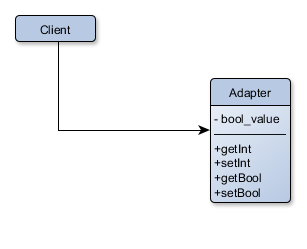
\includegraphics[width=0.6\textwidth]{./Adapter/Class/ClassDiagram.png}
	\caption{Class Adapter: Class Diagram }
	\label{CAclassDiag}
\end{figure}

\begin{itemize}
	\item \textbf{Adaptee}: legacy class with specific methods and fields
	\item \textbf{Target}: desired interface
	\item \textbf{ClassAdapter}: inherits from both Adaptee and Target, adapts the legacy methods to the desired interface  
\end{itemize}

\subsubsection{Fault Model}
Given that the pattern focuses on allowing access to legacy methods through a new interface, failures are found in the following situations:  
\begin{itemize}
	\item the adapter did not inherit from the legacy class or the new interface
	\item the adapter for some reason cannot interact with the legacy methods 
\end{itemize}

\subsection{Testing}
The two sources of failure both depend on the inability of the Client to reach the Adaptee methods through the Adapter.  We reasoned that it is thus sufficient to test the ways in which the variable \textit{bool\_value} interacts and is modified by the methods. As long as the variable changes in an unexpected way the connection between Client and Adaptee is in fact cut off.
\newline
We have thus represented the field's interaction with the class methods through a data flow graph in which the granularity was set such that basic blocks are represented by functions.

We then decided to test the interaction between the variable and the methods following the\textit{ all-uses} criterion, we in fact deemed the\textit{ all-def} criterion not useful to test this pattern because we value mainly the transmission of the right value of the field and thus all its \textit{uses}.    


\paragraph{Data Flow Graph}
 The Client is the only external class interacting with the public methods of the Adapter. The Data Flow Graph can be seen in Figure \ref*{CAdataflow}.
\begin{figure}[h]
	\centering
	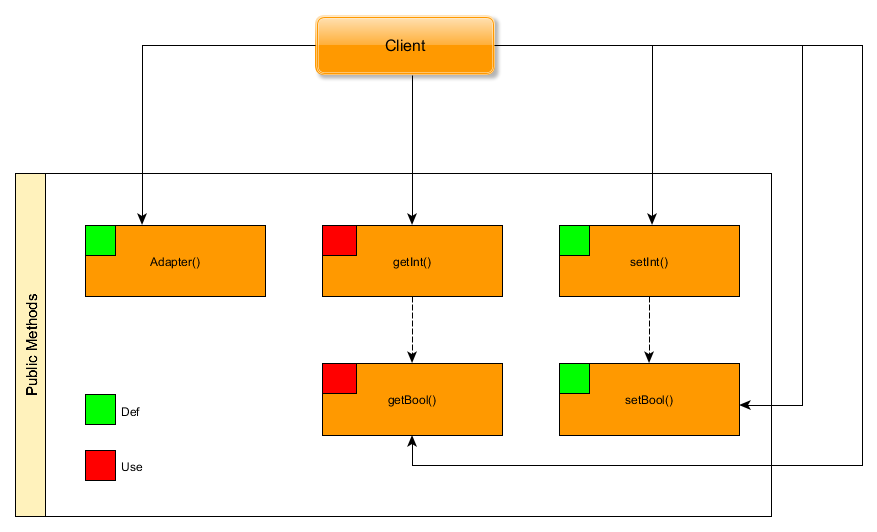
\includegraphics[width=0.8\textwidth]{./Adapter/Class/CallGraph.png}
	\caption{Data Flow Graph: \textit{bool\_value}}
	\label{CAdataflow}
\end{figure}


\subsubsection{Tests}
We generated a test suite capable of testing all the \textit{all-uses} paths:
\begin{itemize}
	\item Adapter() getInt() 
	\item Adapter() getBool() 
	\item Adapter() setInt() getInt() 
	\item Adapter() setInt() getBool() 
	\item Adapter() setBool() getInt()
	\newline
\end{itemize}
The special case of
\begin{itemize}
	\item Adapter() setBool() getBool() 
		
\end{itemize}	
is not tested because all the methods are directly inherited from the legacy class(and thus are supposedly already tested) and no side-effects, which could have invalidated some invariants, are introduced in the adapter.

In this particular pattern the presence of a lone object other than the Client makes Unit and Integration tests un-distinguishable.

\subsubsection{Code Coverage}
The code coverage measure obtained from EclEmma Java plug-in is: 100\%.

%%%%%%%%%%%%%%%%%%%%%%%%%%%%%%%%%%%%%%%%%%%%%1
\section{Object Adapter}
Adapts a pre-existent class to a new interface through class composition. 

Through the new interface the old methods can be directly presented, modified, produce aggregated results or completely new functionality can be added. 

The composition adds the possibility of dynamically switching the adapted legacy class (not contemplated in our implementation) and the possibility of overridden methods with altered functionality.

If the adaptee class is declared final, the increased complexity from overridden methods is eliminated but the extra functionality is removed as well.


\subsubsection{Class Diagram}
\begin{figure}[!h]
	\centering
	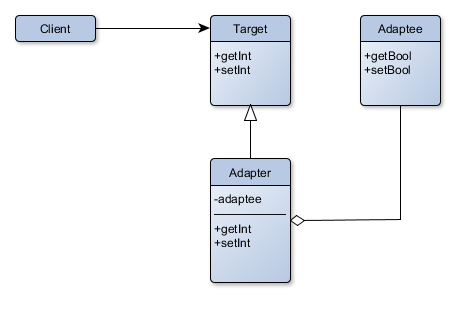
\includegraphics[width=0.7\textwidth]{./Adapter/Object/ClassDiagram.png}
	\caption{Object Adapter: Class Diagram }
	\label{OAclassDiag}
\end{figure}

\begin{itemize}
	\item \textbf{Adaptee}: legacy class with specific methods and fields
	\item \textbf{Target}: desired interface
	\item \textbf{ObjectAdapter}: inherits from Target, adapts the legacy methods to the desired interface through delegation. 
\end{itemize}

\subsubsection{Fault Model}
Given that the pattern focuses on allowing access to legacy methods through a new interface, failures are found in the following situations:  
\begin{itemize}
	\item the adapter did not inherit from the legacy class or the new interface
	\item the adapter for some reason cannot interact with the legacy methods 
	\item the instance contained in the adapter, which inherited the adaptee class, has overrode its methods in an unforeseen way
\end{itemize}


\subsection{Testing}

The sources of failure depend on the inability of the Client to reach the Adaptee methods through the Adapter or in the inability of the Adapter in foreseeing the possible ways in which the Adaptee methods can be overridden:  we reasoned that it is sufficient to test the ways in which the variable \textit{bool\_value} interacts and is modified by the methods, considering all the possible alternative implementations. 
As long as the variable changes in an unexpected way the connection between Client and Adaptee is in fact cut off.

The problem of testing thus expands in two different orthogonal dimensions: data flow, the series of calls that modify or use the variable\textit{bool\_value},  and topology, the different ways the class are ordered in a hierarchy at runtime.

We decided to explore both of them separately in specific focused tests.
\newline
\subparagraph{Data flow}
We have represented the field's interaction with the class methods through a data flow graph in which the granularity was set such that basic blocks are represented by functions.

We then decided to test the interaction between the variable and the methods following the\textit{ all-uses} criterion, we in fact deemed the \textit{all-def} criterion not useful to test this pattern because we value mainly the transmission of the right value of the field and thus all its \textit{uses}.   
\subparagraph{Topology}
We have tested separately the overridden variants of the methods through simple tests.

We reasoned that such a separation would allow us to sufficiently cover the code while maintaining a low number of tests.


\paragraph{Data Flow Graph}
Like the ClassAdapter, only the Client interacts with the Adapter methods.
The Data Flow Graph can be seen in Figure \ref*{OAdataflow}.
\begin{figure}[!h]
	\centering
	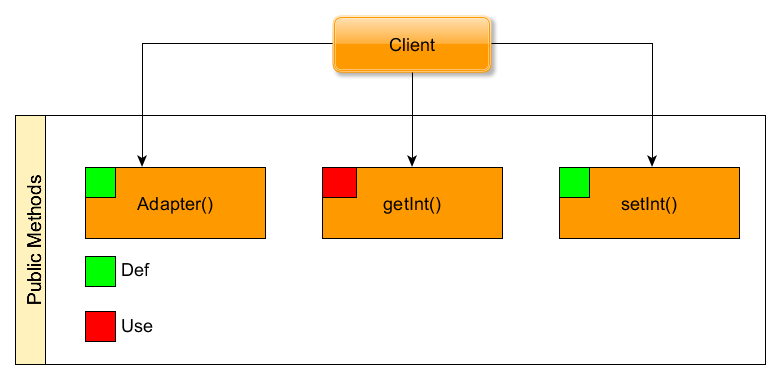
\includegraphics[width=0.8\textwidth]{./Adapter/Object/CallGraph.png}
	\caption{Data Flow Graph: \textit{bool\_value}}
	\label{OAdataflow}
\end{figure}


\subsubsection{Tests}



We generated a test suite capable of testing all the \textit{all-uses} paths:
\begin{enumerate}
	\item Adapter() getInt() 
	\item Adapter() setInt() getInt() 
	
\end{enumerate}
To these are also added the topology tests:
\begin{enumerate}
	\item Adapter( Adaptee ) getInt() 
	\item Adapter( AdapteeOpposite ) getInt()
\end{enumerate}	
Of these the first, being already tested in the first suite, is not repeated.

Since in this pattern the tested class's methods (Adapter's) interacted with external classes (Adaptee) we  differentiated between Unit and Integration tests.

We utilized Mockito's \textit{mock} function to isolate errors with an origin in external classes from interfering with the Adapter class's code.
\subsubsection{Code Coverage}
The code coverage measure obtained from EclEmma Java plugin is: 98.6\% 
\begin{itemize}
	\item Adapter: 97.1\% (UnitTest: 97.1\%)
	\item Adaptee: 100\%
	\item AdapteeOpposite: 100\% 
\end{itemize}

The single remaining untested branch is a setter method which was not called with all the possible inputs equivalence classes.

Since the Unit Tests and the Integration Tests are identical, with the only difference that the Unit Tests utilize Mockito's help to isolate from external classes, the coverage of the Adapter class's code is the same.

%%%%%%%%%%%%%%%%%%%%%%%%%%%%%%%%%%%%%%%%%%%%%2

\section{Proxy}

%%%%%%%%%%%%%%%%%%%%%%%%%%%%%%%%%%%%%%%%%%%%%3
\section{Decorator}

%%%%%%%%%%%%%%%%%%%%%%%%%%%%%%%%%%%%%%%%%%%%%4
\section{Composite}


The Composite pattern allows the creation of hierarchies of composite elements. These composite elements can be composed of single parts or other composite elements.

The Composite pattern "composes" objects into tree structures to represent part-whole hierarchies. Implementing the composite pattern lets clients treat individual objects and compositions uniformlydescribes that a group of objects is to be treated in the same way as a single instance of an object. The intent of a composite is to 

The pattern is useful when there is a need to:
\begin{itemize}
	\item represent hierarchies of 
\end{itemize} 

onsente la costruzione di gerarchie di oggetti composti. Gli oggetti
composti possono essere conformati da oggetti singoli, oppure da altri
oggetti composti. Questo pattern � utile nei casi in cui si vuole:
- Rappresentare gerarchie di oggetti tutto-parte.
- Essere in grado di ignorare le differenze tra oggetti singoli e oggetti
composti.
consente la costruzione di gerarchie di oggetti composti

- operation() su strutture particolari non funziona
-(2) add e remove si comportano in maniera non conforme se applicati: errore su Leaf ed errori su vettore di Composite 



\subsubsection{Class Diagram}
\begin{figure}[!h]
	\centering
	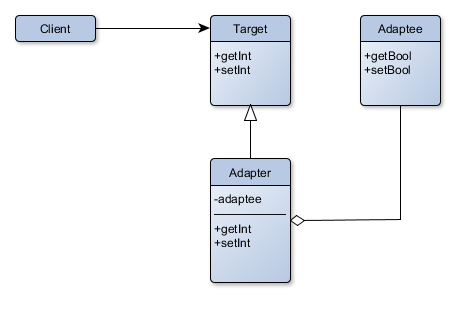
\includegraphics[width=0.7\textwidth]{./Adapter/Object/ClassDiagram.png}
	\caption{Object Adapter: Class Diagram }
	\label{OAclassDiag}
\end{figure}

\begin{itemize}
	\item \textbf{Adaptee}: legacy class with specific methods and fields
	\item \textbf{Target}: desired interface
	\item \textbf{ObjectAdapter}: inherits from Target, adapts the legacy methods to the desired interface through delegation. 
\end{itemize}

\subsubsection{Fault Model}
Given that the pattern focuses on allowing access to legacy methods through a new interface, failures are found in the following situations:  
\begin{itemize}
	\item the adapter did not inherit from the legacy class or the new interface
	\item the adapter for some reason cannot interact with the legacy methods 
	\item the instance contained in the adapter, which inherited the adaptee class, has overrode its methods in an unforeseen way
\end{itemize}


\subsection{Testing}

The sources of failure depend on the inability of the Client to reach the Adaptee methods through the Adapter or in the inability of the Adapter in foreseeing the possible ways in which the Adaptee methods can be overridden:  we reasoned that it is sufficient to test the ways in which the variable \textit{bool\_value} interacts and is modified by the methods, considering all the possible alternative implementations. 
As long as the variable changes in an unexpected way the connection between Client and Adaptee is in fact cut off.

The problem of testing thus expands in two different orthogonal dimensions: data flow, the series of calls that modify or use the variable\textit{bool\_value},  and topology, the different ways the class are ordered in a hierarchy at runtime.

We decided to explore both of them separately in specific focused tests.
\newline
\subparagraph{Data flow}
We have represented the field's interaction with the class methods through a data flow graph in which the granularity was set such that basic blocks are represented by functions.

We then decided to test the interaction between the variable and the methods following the\textit{ all-uses} criterion, we in fact deemed the \textit{all-def} criterion not useful to test this pattern because we value mainly the transmission of the right value of the field and thus all its \textit{uses}.   
\subparagraph{Topology}
We have tested separately the overridden variants of the methods through simple tests.

We reasoned that such a separation would allow us to sufficiently cover the code while maintaining a low number of tests.


\paragraph{Data Flow Graph}
Like the ClassAdapter, only the Client interacts with the Adapter methods.
The Data Flow Graph can be seen in Figure \ref*{OAdataflow}.
\begin{figure}[!h]
	\centering
	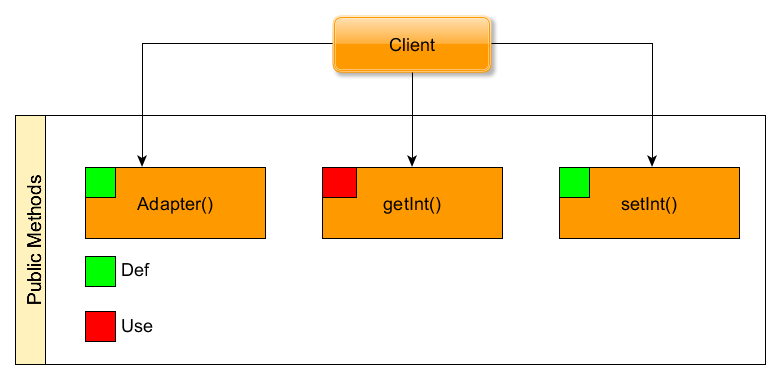
\includegraphics[width=0.8\textwidth]{./Adapter/Object/CallGraph.png}
	\caption{Data Flow Graph: \textit{bool\_value}}
	\label{OAdataflow}
\end{figure}


\subsubsection{Tests}



We generated a test suite capable of testing all the \textit{all-uses} paths:
\begin{enumerate}
	\item Adapter() getInt() 
	\item Adapter() setInt() getInt() 
	
\end{enumerate}
To these are also added the topology tests:
\begin{enumerate}
	\item Adapter( Adaptee ) getInt() 
	\item Adapter( AdapteeOpposite ) getInt()
\end{enumerate}	
Of these the first, being already tested in the first suite, is not repeated.

Since in this pattern the tested class's methods (Adapter's) interacted with external classes (Adaptee) we  differentiated between Unit and Integration tests.

We utilized Mockito's \textit{mock} function to isolate errors with an origin in external classes from interfering with the Adapter class's code.
\subsubsection{Code Coverage}
The code coverage measure obtained from EclEmma Java plugin is: 98.6\% 
\begin{itemize}
	\item Adapter: 97.1\% (UnitTest: 97.1\%)
	\item Adaptee: 100\%
	\item AdapteeOpposite: 100\% 
\end{itemize}

The single remaining untested branch is a setter method which was not called with all the possible inputs equivalence classes.

Since the Unit Tests and the Integration Tests are identical, with the only difference that the Unit Tests utilize Mockito's help to isolate from external classes, the coverage of the Adapter class's code is the same.

-A � di tipo variabile/complessit� dovuta a topologia, rappresentato la nostra microarchitettura tramite  Data Flow graph/Class Dependency graph abbiamo deciso  di utilizzare il criterio di copertura all uses(rispetto a all defs)/all edges(rispetto a all nodes) 
-B � di tipo K,...

%%%%%%%%%%%%%%%%%%%%%%%%%%%%%%%%%%%%%%%%%%%%%5
\section{Observer}

%%%%%%%%%%%%%%%%%%%%%%%%%%%%%%%%%%%%%%%%%%%%%6
\section{State}

%%%%%%%%%%%%%%%%%%%%%%%%%%%%%%%%%%%%%%%%%%%%%7
\section{Visitor}

%%%%%%%%%%%%%%%%%%%%%%%%%%%%%%%%%%%%%%%%%%%%%8

\chapter{JUnit \& Mockito}

\section{JUnit}
\section{Mockito}
\paragraph{EclEmma}
EclEmma is a plug-in which measures the branch coverage of the bytecode produced by the compiler. The branches which were not tested are then traced back to the code and highlighted as a warning. 

In some cases such highlighting is confusing and can even be impossible to eliminate through testing: the Java compiler in fact sometimes creates additional bytecode that seems to have no relation to the source code (e.g. synthetic classes and methods). 

In some other cases test execution is questionable or impossible by design: for example private, empty default constructors (assuming they receive no calls) or methods that contains no logic, like plain getters and setters,
or even extra exception handlers installed to close resources from try/with statements.

\chapter{Conclusioni}

In questo elaborato abbiamo mostrato un sistema in grado di riconoscere automaticamente i muri di una planimetria, indipendentemente dalla notazione grafica utilizzata. In questo programma, se i muri rientrano nelle tipologie citate, � indipendente dagli altri standard e non necessita di informazioni aggiuntive per svolgere il proprio compito.
Dalla bont� dei risultati mostrati nel paragrafo precedente si pu� notare che quello presentato � un metodo valido per l'individuazione di muri in planimetrie. Le idee di base, in parte ispirate agli articoli \cite{1} e \cite{5} e in parte sviluppate ex novo, si sono dimostrate valide per raggiungere l'obiettivo prefissato. A sostegno di quanto appena detto viene ricordato quanto riportato nel capitolo precedente: ossia il fatto che i nostri risultati sono molto simili a quelli ottenuti da CVC ed in alcuni casi sono risultati anche migliori.
Con l'utilizzo di queste idee appena esposte sarebbe possibile arrivare ad un riconoscimento al 100\% indipendente dagli standard grafici utilizzati solo con un'aggiunta di codice che, riconosciuti i muri non pieni, si limiti a riempirli. Una volta raggiunto questo obiettivo un altro sviluppo futuro potrebbe essere il riconoscimento (gi� effettuato da CVC) di altri elementi strutturali quali porte, finestre e stanze.

\addcontentsline{toc}{chapter}{Bibliografia}
\begin{thebibliography}{99}

\bibitem{1} Lluis-Pere de las Heras, David Fernandez, Ernest Valveny, Josep Llados and Gemma Sanchez, ``Unsupervised Wall Detector in Architectural Floor Plans,'' in 12th International Conference on Document Analysis and Recognition, 2013.

\bibitem{2} P. Dosch, K. Tombre, C. Ah-Soon, and G. Masini, ``A complete system for the analysis of architectural drawings,'' International Journal on Document Analysis and Recognition, vol. 3, pp. 102 \verb0-0 116, 2000.

\bibitem{3} T. Lu, H. Yang, R. Yang, and S. Cai, ``Automatic analysis and integration of architectural drawings,'' International Journal on Document Analysis and Recognition, vol. 9, pp. 31 \verb0-0 47, 2007.

\bibitem{4} S. Mace, H. Locteau, E. Valveny, and S. Tabbone, ``A system to detect rooms in architectural floor plan images,'' in Proceedings of the 9th IAPR International Workshop on Document Analysis Systems, 2010, pp. 167\verb0-0 174.

\bibitem{5} Lluis-Pere de las Heras, David Fernandez, Ernest Valveny, Josep Llados and Gemma Sanchez, ``Statistical segmentation and structural recognition for floor plan interpretation,''  2013.

\bibitem{6} S. Ahmed, M. Liwicki, M. Weber, and A. Dengel, ``Improved automatic analysis of architectural floor plans,'' in Proceedings of the 11th International Conference on Document Analysis and Recognition, 2011.

\end{thebibliography}
\addcontentsline{toc}{chapter}{Elenco delle Figure}\listoffigures
\end{document}
